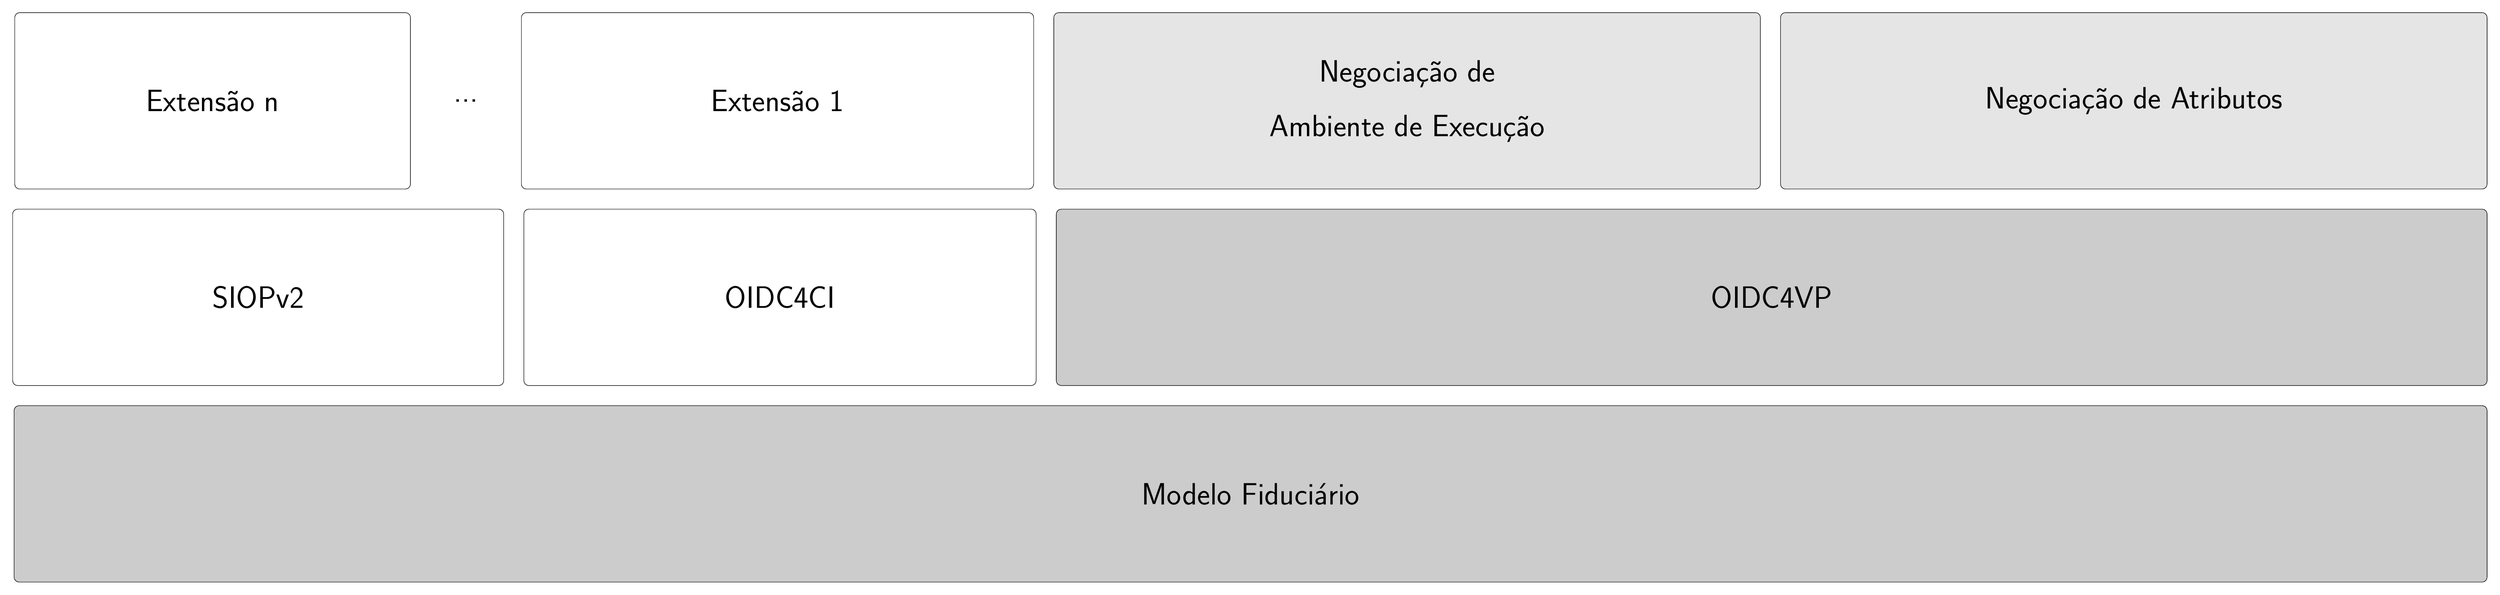
\begin{tikzpicture}[node distance=1cm,outer sep=1pt,inner sep=1pt]

    % CONFIGURANDO OS NODOS 
 
    %------------------------ CAMADA 3----------------------------%
    \tikzset{field/.style={align=center,shape=rectangle,rounded corners,minimum height=5cm,minimum width=20cm,draw,font=\fontsize{36}{44}\selectfont\sffamily,fill=gray!20}}

    \tikzset{field2/.style={align=center,shape=rectangle,rounded corners,minimum height=5cm,minimum width=29cm,draw,font=\fontsize{36}{44}\selectfont\sffamily,fill=gray!20}}

    %------------------------ CAMADA 2----------------------------%
    \tikzset{mediumfield/.style={align=center,shape=rectangle,rounded corners,minimum height=5cm,minimum width=40.5cm,draw,font=\fontsize{36}{44}\selectfont\sffamily,fill=gray!40}}

    \tikzset{mediumfield2/.style={align=center,shape=rectangle,rounded corners,minimum height=5cm,minimum width=14.5cm,draw,font=\fontsize{36}{44}\selectfont\sffamily,fill=gray!40}}

    \tikzset{mediumfield3/.style={align=center,shape=rectangle,rounded corners,minimum height=5cm,minimum width=13.9cm,draw,font=\fontsize{36}{44}\selectfont\sffamily,fill=gray!40}}

 %------------------------ CAMADA 1----------------------------%
    \tikzset{largefield/.style={align=center,shape=rectangle,rounded corners,minimum height=5cm,minimum width=70cm,draw,font=\fontsize{36}{44}\selectfont\sffamily,fill=gray!40}}


    % INSTANCIANDO OS NODOS
    
    %------------------------ CAMADA 1----------------------------%
    % Desenho do primeiro retângulo (grande)
    \node [largefield] (fid) {Modelo Fiduciário};


    %------------------------ CAMADA 2----------------------------%
    % Desenho do segundo retângulo (médio), alinhado à direita com o primeiro, e posicionado acima
    \node [mediumfield,anchor=south east] at ([yshift=0.5cm]fid.north east) (oidc4vp) {OIDC4VP};

     % Desenho do segundo retângulo (médio), alinhado à direita com o primeiro, e posicionado acima
    \node [mediumfield2,anchor=south east, fill=white] at ([xshift=-0.5cm]oidc4vp.south west) (oidc4ci) {OIDC4CI};

    \node [mediumfield3,anchor=south east, fill=white] at ([xshift=-0.5cm]oidc4ci.south west) (siopv2) {SIOPv2};
    %------------------------ CAMADA 3----------------------------%

    \node [field,anchor=south east] at ([yshift=0.5cm]oidc4vp.north east) (atributes) {Negociação de Atributos};
    
    \node [field,anchor=south east] at ([xshift=-0.5cm]atributes.south west) (env) {Negociação de \\ Ambiente de Execução};

    % \node [mediumfield2,anchor=south east, fill=white, minimum width=14cm] at ([xshift=-0.5cm]env.south west) (ext1) {Extensão 1};
    \node [mediumfield2,anchor=south east, fill=white, minimum width=14.5cm] at ([xshift=-0.5cm]env.south west)  (ext1) {Extensão 1};
    \node [mediumfield2,anchor=south east, fill=white, minimum width=2cm, draw=white] at ([xshift=-0.5cm]ext1.south west) (dots) {...};
    \node [mediumfield2,anchor=south east, fill=white, minimum width=11.2cm] at ([xshift=-0.5cm]dots.south west) (extn) {Extensão n};    

    % \node [mediumfield2,anchor=south east, fill=white, draw=white] at ([xshift=-0.5cm]ext1.south west) (env) {\large{...}};
    % \node [field2,anchor=south east] at ([xshift=-0.5cm]env.south west) (aud) {Auditoria};
    
    
    
\end{tikzpicture}